\chapter{Sharing Immutable Data}
\label{chapter:sharing-immutable-data}

So far, we have been concerned with the wasteful overhead that results from
data representation. But what about the data itself? If you examine any Java
heap, you will find that a
large amount of the data is duplicated. At one extreme, 
there are often thousands of copies of the same boxed
integers, especially 0 and 1. At the other extreme, there may be many
 small data
structures that have the same shape and data. 
And, of course, duplicate strings are extremely common.
This chapter describes various
techniques for sharing data to avoid
duplication, including a few low-level mechanisms that Java provides.

\section{String Literals}
\label{sec:literals}

Duplicate strings are not only one of the
most common sources of memory waste, they are also very expensive, since even
small strings incur a large overhead. Fortunately, it is not
hard to eliminate string duplication. 

 One technique is to represent strings as  
literals whenever possible. Duplication problems arise because dynamically
 created \class{String}s
are stored in the heap without checking whether they already
exist. \class{String} literals, on the other hand, are stored in a
\emph{string constant pool} when classes
are loaded, where they are shared. Therefore, there is a big advantage to
\class{String} literals.

 As an example, suppose an application
reads in property name-value pairs from files into tables:
\begin{shortlisting}
class ConfigurationProperties {
    ..
	void handleNextEntry() {
		String propertyName = getNextString();
		String propertyValue = getNextString();
		propertyMap.put(propertyName, propertyValue);
	}
}
\end{shortlisting}
The \class{String}s stored in \code{propertyMap} are created dynamically. If 
there are just a few distinct property names in all of the input pairs, these
property names will be duplicated many times in the heap.

However, if you know in advance what all of the property names are, then you can
define them once as \class{String} literals, which can be shared among the
entries of \code{propertyMap}.
\begin{shortlisting}
class PropertyNames {
	public static String numberOfUnits = ``NUM_UNITS'';
	public static String minWidgets = ``MIN_WIDGETS'';
	..
}

class ConfigurationWithStaticProperties {
    void handleNextEntry() {
       String propertyName = getNextPropertyName(); 
       String propertyValue = getNextString();
       propertyMap.put(propertyName, propertyValue);
    }
}
\end{shortlisting}
The \code{getNextPropertyName} method reads in a property name, and returns
a pointer to a property name literal, stored in the JVM string
constant pool. Alternatively, defining an enumeration
type to encode property names may be a better stylistic choice.

A common
 mistake is to create a new \class{String}  from a \class{String} literal,
 which is usually completely unnecessary:
\begin{shortlisting}
class PropertyNames {
	public static String numberOfUnits = 
	                           new String(``NUM_UNITS'');
	public static String minWidgets = 
	                           new String(``MIN_WIDGETS'');
	..
}
\end{shortlisting}
Even though the standard library is smart enough to share
character arrays in this case, this code still creates redundant \class{String}
objects in the heap.

Using \class{String} literals to avoid dulication is only possible when the
\class{String} values are known in advance. 
Section~\ref{sec:sharing-pools} introduces the notion of a sharing pool for
sharing dynamic data. Section~\ref{sec:sharing-strings} describes the Java
string interning mechanism, which uses a built-in string sharing pool to
eliminate duplication.

\section{Sharing Pools}
\label{sec:sharing-pools}

Suppose an application generates a lot of duplicated data and the values
are unknown before execution. 
You can eliminate data duplication by using a \emph{sharing pool}, as shown
in Figure~\ref{fig:sharing-pool}. In Figure~\ref{fig:sharing-pool}(a), objects
A and B point to identical data structures.
Figure~\ref{fig:sharing-pool}(b) shows objects A and B sharing the same data
structure, which is stored in a sharing pool.
 \begin{figure}
  \centering
 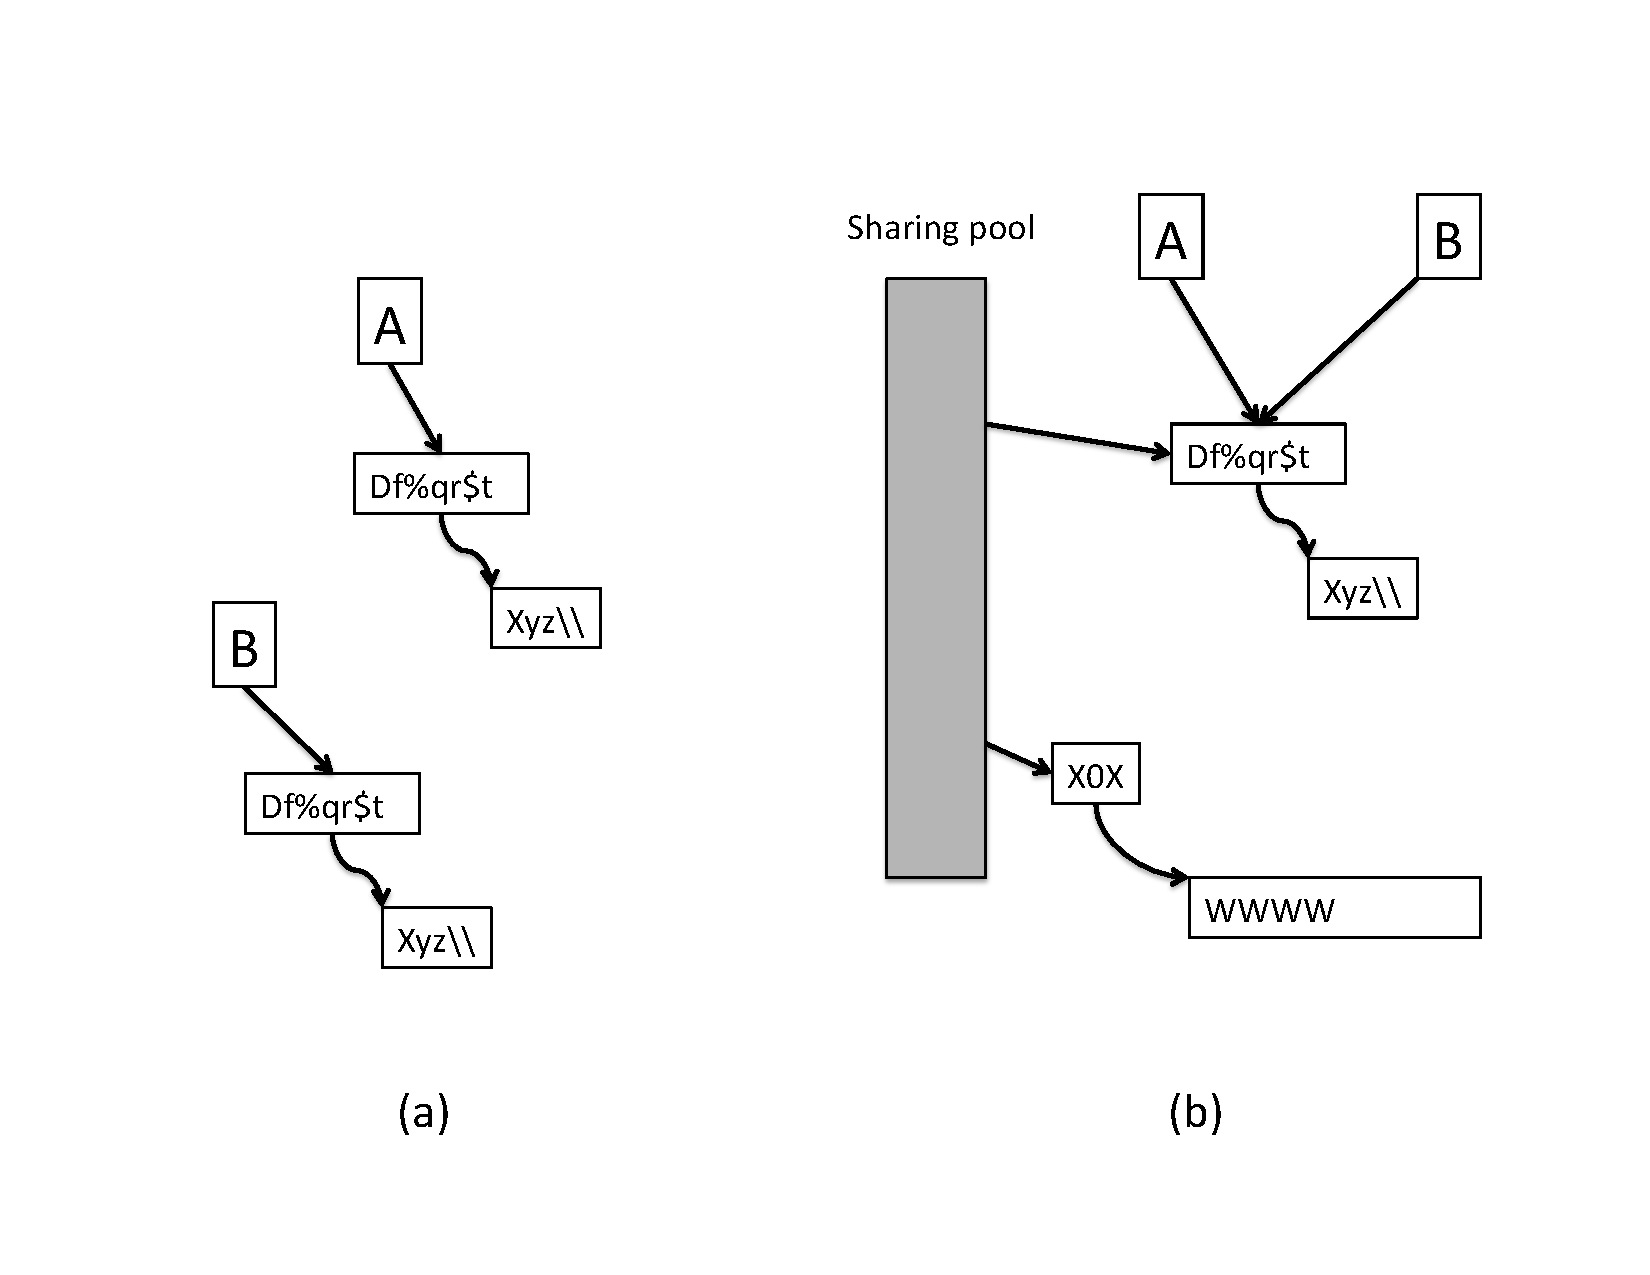
\includegraphics[width=.80\textwidth]{part1/Figures/modelingdatatypes/sharing-pool.pdf}
  \caption{(a) Objects A and B point to duplicate data. (b) Objects A and B
  share the same data, stored in a sharing pool.}
  \label{fig:sharing-pool}
\end{figure}

\callout{callout:sharing-pool}{Sharing Pool}{
A \emph{sharing pool} is a centralized structure that stores 
canonical data values that would otherwise be replicated in many objects.
A sharing pool itself is usually some sort of hash table, although it
could be implemented in other ways.
}

There are several issues that you need to be aware of before using a sharing
pool.
\paragraph{Shared objects must be immutable.} Changing shared data can
have unintended side effects. For example, 
changing A in Figure~\ref{fig:sharing-pool}(b), 
also changes the value of B.

\paragraph{The result of equality testing should be the same, whether or
not objects are shared.}
 In particular, you should never use \code{==} on shared objects.
In Figure~\ref{fig:sharing-pool}, \code{A == B} is false in
Figure~\ref{fig:sharing-pool}(a) and true in Figure~\ref{fig:sharing-pool}(b),
 which can lead to very subtle bugs. It is dangerous to use \code{==} in any
 case, unless exact object identity is really required.
 
\paragraph{Sharing pools should not be used if there is limited sharing.}
A sharing pool itself adds
memory costs, including additional per-entry costs. If there is not
much sharing, then the memory saved from
eliminating duplicates isn't enough to compensate for the
extra cost, and memory will be wasted instead of saved.

% NMM 20110614 i thought this was a good idea, but in Java, a reference will
% always be cheaper than an object, because of the header!
%\paragraph{The shared data items must be sufficiently large.} The size of the
%each pooled data item must be large, relative to the cost of a reference ---
%when using a pool, you still need to pay at least one reference cost for
%each use of the pooled items. 

\paragraph{Shared objects should be garbage collected.}
In Figure~\ref{fig:sharing-pool}(b), the sharing pool stores an object
that no other object is pointing to. Over time, the sharing pool can fill up
with garbage, that is, items that were once needed but not any more. If the
sharing pool is not purged of these unused items, there is a memory
leak that can eventually use up all of memory.

Fortunately, Java provides a few built in mechanisms that take care of some of
these concerns.

\section{String Interning}
\label{sec:sharing-strings}
\index{Interning}

%Before storing a 
%To use a sharing pool, before storing a new
%\class{String}, first check the pool to see if it is already there. If it is,
%reuse it; otherwise, add the new string to the pool. 
%One catch is that if you end up adding many strings to
%the pool that are never reused, then you will waste memory, since the pool
%structure itself has overhead. So you need to have a good idea
%which strings are likely to have duplicate values.

 Since \class{String} duplication is so common, Java provides a built-in string
 pool for sharing \class{String}s, implemented by the native JVM and maintained in
 its internal \emph{perm space}. To share a \class{String}, you simply call the
 method \code{intern} on it, and everything is taken care of automatically.
Since \class{String}s are immutable, sharing is safe. However, the rule about
not using \code{==} still holds on shared \class{String}s.
  
In the example from section~\ref{literals},
\class{ConfigurationWithStaticProperties} eliminates property
name duplication but not
property value duplication. Suppose you know that there are
not too many distinct values, but you don't know what they are. In this case,
property values are perfect candidates for interning.
\begin{shortlisting}
 
 class ConfigurationPropertiesWithInterning {
    void handleNextEntry() {
       PropertyName propertyName = getNextPropertyName(); 
       String propertyValue = getNextString().intern();
       propertyMap.put(propertyName, propertyValue);
    }
}
\end{shortlisting}

The call to \code{intern} adds the new property value \class{String}
 to the internal string
pool if it isn't there already, and return a pointer to it. Otherwise, the
new \class{String} is a duplicate, and a previously saved \class{String} is
returned.

Even though interned \class{String} are not stored in the heap, they do incur
native memory overhead, and native memory is not free.
 Interning \class{String}s indiscriminately wastes memory and can result in an
 exception: \code{java.lang.OutOfMemoryError:PermGen Space}. 
There are JVM parameters to adjust the perm space size:
\code{-XX:PermSize=128m} sets perm size to 128 megabytes, and
\code{-XX:MaxPermSize=512m} sets the maximum perm size to 512 megabytes.
\index{Permspace Heap}
Fortunately, the JVM performs garbage collection on the internal string pool, so there is no danger of a memory leak.

TODO: shorten this to a quick forward reference. There is an
important variant of a sharing pool called the Bulk Sharing Pool. Like a normal sharing pool, the goal of a bulk sharing pool is to amortize the
memor costs of storing data. However, rather than mitigate the costs of data
duplication, a bulk sharing pool aims to amortize the costs of Java object
headers across the elements in a pool. This is a topic that stretches notions of
how to store data beyond the normal Java box, and so will be discussed, along
with many similar matters, in \autoref{chapter:large-long-lived}.

 %    * Literal strings within the same class in the same package represent
%     references to the same String object. * Literal strings within different
 %    classes in the same package represent references to the same String
%     object. * Literal strings within different classes in different packages
 %    likewise represent references to the same String object. * Strings
 %    computed by constant expressions are computed at compile time and then
   %  treated as if they were literals. * Strings computed by concatenation at
    % run time are newly created and therefore distinct.
\section{Integer Sharing Pool}

As of \javafive, the Java library provides a sharing pool for \class{Integer}s.
Unlike the string pool, the \class{Integer} pool is initialized at class load
time to store all \class{Integer}s in a fixed range, from -128 to 127 by
default. The method \code{Integer.valueOf(int value)} returns a pointer to an
\class{Integer} in the pool, provided \code{value} is in range.

\begin{wrapfigure}{r}{0.4\textwidth}
\centering
\begin{framedlisting}
for (int i=1; i<=50; i++) {
 numbers[i] = Integer.valueOf(i);
}
\end{framedlisting}
\caption{By using the \code{valueOf} method, you can leverage the standard
library's integer sharing pool.}
\label{fig:integer-sharing-pool}
\end{wrapfigure}
Because the \class{Integer} sharing pool is pre-initialized and fixed in size,
it's always a good idea to call \code{Integer.valueOf} instead of the
constructor to create a new \class{Integer}. For example, the code in
\autoref{fig:integer-sharing-pool} stores \class{Integer}s from 1 to 50 in an
array. Unless you tweak things from the command line,
\code{valueOf} returns an existing \class{Integer}
for the first 127 numbers, and, for the rest of the numbers, \code{valueOf}
returns a new \class{Integer} instance. You should always make use of
\class{Integer.valueOf}: the pooling aspect is very cheap, and you never have to
worry about wasting memory. You do have to be careful, however, to avoid using
\code{==} to compare potentially shared \class{Integer}s. The documentation for
\class{Integer} does not specify anything about the default range of pooled
values, and so you may be in for a surprise if you start assuming that
\code{Integer.valueOf(100) == Integer.valueOf(100)}.

There is a JVM parameter to change the size of the \class{Integer} sharing pool.
By adding \code{-XX:AutoBoxCacheMax=100} to your applicaiton's command line, the
pooled integers will range over the values 0 to 100.

\section{Canonicalizing Maps: Sharing General Objects}

Beyond strings and boxed \class{Integer}s, there are often other kinds of
duplicated objects and data structures consuming large portions of the heap. 
There is no built-in Java mechanism to share objects or data
structures in general, so you have to implement a sharing pool for them from
scratch. All of the sharing pool issues from Section~\ref{sec:sharing-pools} need to be
addressed. The shared objects or structures must be immutable, they must not be
compared using \code{==}, there must be sufficient memory savings from sharing
to justify the sharing pool, and the sharing pool must be not cause a memory leak. 
Note that, unless overridden, \code{equals} is
implemented as \code{==}, so sharing data structures typically requires writing
a new \code{equals} method.

To illustrate a user-written sharing pool, consider a graph where the nodes
have annotations, many of which are duplicates. Both the graph and the
annotations are modified dynamically. The two basic requirements are 1) the
ability to find existing annotations quickly to share them, and 2) the ability
to release annotations that are no longer associated with any node, so they can
be garbage collected.  The second requirement prevents a memory leak. 

\begin{wrapfigure}{r}{0.5\textwidth}
\centering
\begin{framedlisting}
HashMap<Annotation, Annotation> canoncalizingMap;
\end{framedlisting}
\end{wrapfigure}
Interestingly, none of the common collection classes meet these requirements
out-of-the-box. A \class{HashSet} can store \class{Annotation}s uniquely, but
retrieving an existing \class{Annotation} is not easy. The \class{HashSet}
implementation can only speedily let you know whether an equivalent item already
exists in the set, but can not return that existing item. To get the preexisting
item, you would need to iterate over the entire set. Therefore, the first
requirement is best implemented as a \class{HashMap} mapping an
\class{Annotation}s to the canonical instance, as shown on the right. A common
term for this structure is a \emph{canonicalizing map}.
\index{Canonicalizing Map}

A \class{HashMap} largely suits the role of a canonicalizing map. However, it is
still possible to have memory issues, either because stale entries persist in
the map, or because the map grows without bound.
\autoref{sec:sharing-pools-safety} discusses how to avoid these issues, by using
some more advanced features of Java.

\section{Summary} 

Not only are Java heaps bloated from too much overhead, they
are also bloated from duplicated data. If you know that your application
generates many copies of the same data, then you should find a way to share the
data. Java provides several built-in sharing mechanisms:

\begin{itemize}
  \item The JVM maintains a native sharing
  pool for \class{Strings}. Use \class{String} interning to make use of this
  sharing pool.
  \item The standard library maintains a fixed size pool for
   a fixed range of  \class{Integer}s. You should use \code{valueOf} to create
   \class{Integer}s instead of a constructor.
\end{itemize}
Additionally, Java provides a weak referencing mechanism, which can be used to
implement your own sharing pool.

These mechanisms appear to be clumsy addons that were necessary to solve
problems that came up in practice. But they are better than nothing, and
without them, it would be much harder to share data. 
Whether or not you use these mechanisms, you should remember these four rules:
\begin{itemize}
  \item Shared objects must be immutable.
  \item The result of equality testing should be the same, whether or
not objects are shared.  
  \item Sharing pools should not be used if there is limited sharing.
  \item Shared objects should be garbage collected.
\end{itemize}





